% Informe en formato IEEE (conferencia, dos columnas).
% Compilar desde esta carpeta:  pdflatex informe.tex (dos pasadas)
% IEEEtran.cls está incluido al lado para no depender de la instalación de TeX.

\documentclass[conference,a4paper]{IEEEtran}

\usepackage[utf8]{inputenc}
\usepackage[T1]{fontenc}
\usepackage{mathptmx}
\usepackage{amsmath,amssymb}
\usepackage{graphicx}
\usepackage{booktabs}
\usepackage{array}
\usepackage{xcolor}
\usepackage{listings}
\usepackage{enumitem}
\setlist{noitemsep,topsep=2pt,leftmargin=*}
\usepackage{tikz}
\usetikzlibrary{positioning,arrows.meta,fit,calc}
\usepackage[hidelinks]{hyperref}

% IEEEtran trae los rótulos en inglés y no hay babel-spanish instalado.
\renewcommand{\abstractname}{Resumen}
\renewcommand{\IEEEkeywordsname}{Palabras clave}
\renewcommand{\tablename}{TABLA}
\renewcommand{\refname}{Referencias}
\renewcommand{\lstlistingname}{Listado}

\lstset{
  basicstyle=\ttfamily\scriptsize,
  keywordstyle=\bfseries,
  columns=fullflexible,
  breaklines=true,
  keepspaces=true,
  frame=tb,
  framesep=2.5pt,
  xleftmargin=1.5pt,
  aboveskip=4pt,
  belowskip=4pt,
  literate={á}{{\'a}}1 {é}{{\'e}}1 {í}{{\'i}}1 {ó}{{\'o}}1 {ú}{{\'u}}1 {ñ}{{\~n}}1
}

% Sin patrones de español: se cortan a mano las palabras largas más frecuentes.
\hyphenation{par-ti-cio-nes pro-ce-sa-mien-to dis-tri-bui-do dis-tri-bui-dos
  i-te-ra-cio-nes cen-troi-de cen-troi-des e-je-cu-tor e-je-cu-to-res
  a-gru-pa-mien-to me-mo-ria trans-for-ma-cio-nes es-pe-cu-la-ti-va
  a-pli-ca-cio-nes al-go-rit-mo al-go-rit-mos ac-ti-vi-dad pro-yec-tor
  ce-lu-lar ce-lu-la-res es-tu-dian-tes per-sis-ten-cia bi-blio-te-ca
  a-pren-di-za-je par-ti-cio-na-mien-to ca-na-li-za-cio-nes ca-na-li-za-ci-on
  je-rar-qui-ca je-rar-qui-co se-ria-li-za-ci-on op-ti-mi-za-dor
  op-ti-mi-za-do-res pre-di-ca-do pre-di-ca-dos con-ve-xen-cia e-va-lua-dor
  re-la-cio-na-les re-la-cio-nal con-ver-gen-cia es-ta-dis-ti-co
  es-ta-dis-ti-cos car-di-na-li-dad di-men-sio-na-li-dad trans-for-ma-dor
  trans-for-ma-do-res es-ti-ma-dor es-ti-ma-do-res}

\begin{document}

\begin{titlepage}
\thispagestyle{empty}
\centering
\vspace*{2cm}
{\Large\bfseries ITS Villada\par}
\vspace{0.5cm}
{\large Base de Datos II\par}
\vfill
{\large\bfseries INFORME DE INVESTIGACIÓN\par}
\vspace{0.6cm}
{\large Grupo N° 8\par}
\vspace{1.5cm}
{\LARGE\bfseries Procesamiento distribuido y \textit{machine learning}\\
sobre datos masivos con Apache Spark MLlib\par}
\vspace{0.5cm}
{\large Arquitectura, Algoritmos Iterativos y Optimización a Gran Escala\par}
\vfill
{\large\bfseries Integrantes\par}
\vspace{0.25cm}
Leon Guchea\\
Bautista Daveloze\\
Riccioni Santiago\\
Sibona Luciano\\
Macias Luciano
\vspace{0.8cm}

{\large\bfseries Docentes\par}
\vspace{0.25cm}
Lisandro Márquez\\
Teodoro Reyna
\vfill
{\large 11 de noviembre de 2026\par}
\vspace*{1cm}
\end{titlepage}
\pagenumbering{arabic}
\setcounter{page}{1}
\pagestyle{plain}

\begin{abstract}
Cuando el volumen de un conjunto de datos excede las capacidades de almacenamiento y cómputo de un único servidor, su análisis exige estrategias de particionamiento horizontal y procesamiento paralelo en clúster. Este informe examina los principios arquitectónicos y algorítmicos del procesamiento distribuido moderno, analizando la transición desde el paradigma MapReduce hacia el modelo en memoria de Apache Spark, sus RDD, DataFrames y el optimizador Catalyst. Se profundiza en el funcionamiento de Spark MLlib para el aprendizaje automático sobre datos masivos, adoptando el algoritmo de agrupamiento K-Means como caso de estudio representativo de algoritmos iterativos. Se analizan formalmente la paralelización mediante estadísticos suficientes, la agregación jerárquica en árbol (\textit{treeAggregate}), las canalizaciones (\textit{ML Pipelines}), los mecanismos de tolerancia a fallos por linaje y la mitigación de tareas rezagadas mediante ejecución especulativa. Asimismo, se contrasta el procesamiento analítico distribuido con las bases de datos relacionales tradicionales y se detallan las técnicas críticas de optimización del motor (Project Tungsten, gestión de memoria fuera de la JVM) y la resolución de cuellos de botella por sesgo de datos (\textit{data skew}) y operaciones de \textit{shuffle}.
\end{abstract}

\begin{IEEEkeywords}
Apache Spark, MLlib, MapReduce, Hadoop, K-Means, procesamiento distribuido, RDD, tolerancia a fallos, big data, Catalyst, Project Tungsten, treeAggregate.
\end{IEEEkeywords}

\section{Introducción}

El volumen de datos que generan hoy las organizaciones (registros transaccionales, eventos de aplicaciones, telemetría de sensores y flujos de interacción en tiempo real) crece a un ritmo superior a la capacidad de una única máquina para almacenarlos y procesarlos. Ante este límite físico existen dos caminos: escalar verticalmente (\textit{scale-up}), adquiriendo servidores con mayor cantidad de núcleos y memoria, o escalar horizontalmente (\textit{scale-out}), distribuyendo el conjunto de datos y la carga de cómputo entre múltiples computadoras conectadas en red. La vía horizontal resulta económicamente viable y no posee un techo rígido de hardware, pero introduce retos complejos de sistemas distribuidos: división coherente de datos, coordinación inter-nodo, sobrecarga en la red (\textit{network traffic}) y preservación de consistencia ante fallos parciales de hardware.

Google formalizó una primera respuesta masiva a estos problemas con el modelo MapReduce~\cite{dean2004mapreduce}, que el ecosistema Apache popularizó a través de Hadoop y su sistema de archivos distribuido HDFS~\cite{shvachko2010hdfs}. Si bien MapReduce resultó altamente robusto y eficaz para transformaciones por lotes de una sola pasada, evidenció severas ineficiencias en algoritmos iterativos característicos del aprendizaje automático (\textit{Machine Learning}), los cuales requieren recorrer las mismas estructuras de datos decenas de veces. Apache Spark~\cite{zaharia2010spark,zaharia2012rdd} surgió específicamente para resolver esta deficiencia, conservando los datos intermedios en memoria entre iteraciones y garantizando tolerancia a fallos sin recurrir a la replicación en disco.

Este informe tiene dos objetivos principales:
\begin{enumerate}
\item Analizar los fundamentos teóricos y la arquitectura de Apache Spark y de su biblioteca de aprendizaje automático, MLlib~\cite{meng2016mllib}, contrastando su paradigma distribuido y analítico con el procesamiento de las bases de datos relacionales tradicionales.
\item Estudiar en profundidad la paralelización de algoritmos iterativos sobre macrodatos, tomando como núcleo analítico a K-Means, y examinando los patrones de agregación jerárquica (\textit{treeAggregate}), las canalizaciones (\textit{ML Pipelines}), las optimizaciones de bajo nivel del motor (Catalyst y Project Tungsten) y las estrategias para resolver cuellos de botella en producción.
\end{enumerate}

El resto del informe se estructura de la siguiente manera: la Sección~\ref{sec:marco} expone el marco teórico del procesamiento distribuido y la arquitectura de Spark; la Sección~\ref{sec:relacional} examina los casos de uso y compara Spark con los sistemas relacionales; la Sección~\ref{sec:kmeans} formaliza el algoritmo K-Means y su paralelización mediante estadísticos suficientes; la Sección~\ref{sec:fallos} analiza la tolerancia a fallos por linaje, la ejecución especulativa y la comparación temporal analítica con Hadoop; la Sección~\ref{sec:mllib-avanzado} profundiza en el aprendizaje automático a escala masiva, agregación en árbol, canalizaciones, optimizaciones del motor y mitigación de cuellos de botella; finalmente, la Sección~\ref{sec:conclusiones} resume las conclusiones.

\section{Marco teórico}
\label{sec:marco}

\subsection{El modelo MapReduce}

MapReduce~\cite{dean2004mapreduce} estructura cualquier cómputo distribuido sobre dos funciones parametrizadas por el desarrollador. La función \textit{map} procesa de manera aislada y paralela cada fragmento de la entrada, emitiendo pares clave--valor intermedios. Posteriormente, el entorno de ejecución agrupa todos los valores asociados a una misma clave y los distribuye a través de la red en una fase denominada \textit{shuffle}. Finalmente, la función \textit{reduce} procesa la lista agregada de valores para cada clave, generando la salida consolidada. De manera complementaria, una función local \textit{combiner} puede aplicar una reducción previa en cada nodo antes del \textit{shuffle}, disminuyendo drásticamente el tráfico cuando la operación es asociativa y conmutativa.

El sistema subyacente se encarga de particionar la entrada, planificar tareas, reintentar ejecuciones fallidas y supervisar la red. Para asegurar resiliencia absoluta, cada etapa de MapReduce lee sus entradas desde HDFS y almacena sus salidas en disco con replicación triple~\cite{shvachko2010hdfs}. Si bien este mecanismo garantiza alta tolerancia a fallos, impone una penalización de rendimiento prohibitiva en algoritmos iterativos: cada paso sucesivo debe encadenar un trabajo independiente que paga el costo de escribir y volver a leer del disco todo el conjunto de datos.

\subsection{Apache Spark y los RDD}

Spark~\cite{zaharia2010spark} supera esta barrera mediante el concepto de \textit{Resilient Distributed Dataset} (RDD)~\cite{zaharia2012rdd}: una colección distribuida, inmutable y particionada de objetos en memoria. Sobre los RDD se definen dos categorías de operaciones:

\begin{itemize}
\item \textbf{Transformaciones} (\texttt{map}, \texttt{filter}, \texttt{groupByKey}, \ldots): Definen un nuevo RDD aplicando una función sobre uno existente. Son de evaluación perezosa (\textit{lazy evaluation}): no se calculan al invocarse, sino que se ensamblan en un grafo dirigido acíclico (DAG) que describe el linaje lógico de cómputo.
\item \textbf{Acciones} (\texttt{count}, \texttt{collect}, \texttt{reduce}, \ldots): Requieren materializar un resultado hacia el \textit{driver} o escribirlo en almacenamiento, lo que desencadena la optimización y ejecución efectiva del DAG.
\end{itemize}

La evaluación perezosa permite que el planificador inspeccione el grafo de ejecución completo antes de despachar tareas. De este modo, Spark clasifica las dependencias en dos tipos:
\begin{enumerate}
\item \textit{Dependencias estrechas} (\textit{narrow}): Cada partición del RDD padre es utilizada por a lo sumo una partición del RDD hijo (ej. \texttt{map}, \texttt{filter}). Permiten ejecutar múltiples operaciones encadenadas en memoria dentro del mismo hilo (\textit{pipelining}) sin sincronización por red.
\item \textit{Dependencias amplias} (\textit{wide}): Múltiples particiones hijas dependen de datos distribuidos en distintas particiones padres (ej. \texttt{reduceByKey}, \texttt{join}). Requieren una costosa etapa de \textit{shuffle} y delimitan las fronteras entre etapas (\textit{stages}) de ejecución.
\end{enumerate}

Dos propiedades diferencian decisivamente a los RDD. La primera es la \textbf{persistencia explícita}: mediante \texttt{cache()} o \texttt{persist()}, el programador puede mantener un RDD materializado en la memoria RAM de los nodos trabajadores tras su primera evaluación, permitiendo su reutilización en decenas de iteraciones sin incurrir en I/O de almacenamiento. La segunda es el \textbf{linaje} (\textit{lineage}): en lugar de mantener copias redundantes de conjuntos intermedios en disco, cada partición retiene la fórmula exacta de transformaciones que la originaron. Ante la pérdida de un nodo, Spark simplemente reejecuta las transformaciones sobre la partición afectada desde la fuente persistente~\cite{zaharia2012rdd}.

\subsection{Arquitectura de ejecución}

Una aplicación en Apache Spark se compone de cuatro entidades estructurales~\cite{spark-cluster}, representadas esquemáticamente en la Fig.~\ref{fig:arquitectura}:

\begin{itemize}
\item \textbf{Driver}: Proceso principal que ejecuta la función \texttt{main} del programa. Traduce el código a un grafo DAG, descompone el plan en etapas y tareas, programa su ejecución y consolida resultados finales.
\item \textbf{Cluster Manager} (o \textit{master}): Administra la asignación de recursos computacionales físicos o virtualizados en el clúster. Puede operar en modo nativo (\textit{Standalone}), YARN~\cite{vavilapalli2013yarn} o Kubernetes.
\item \textbf{Worker Node}: Servidor físico o máquina virtual perteneciente al clúster, responsable de alojar y mantener procesos ejecutores.
\item \textbf{Executor}: Proceso independiente instanciado en un \textit{worker} para una aplicación específica. Ejecuta tareas concurrentes en hilos sobre particiones de datos y conserva fragmentos de RDD persistidos en su espacio de memoria.
\end{itemize}

\begin{figure}[t]
\centering
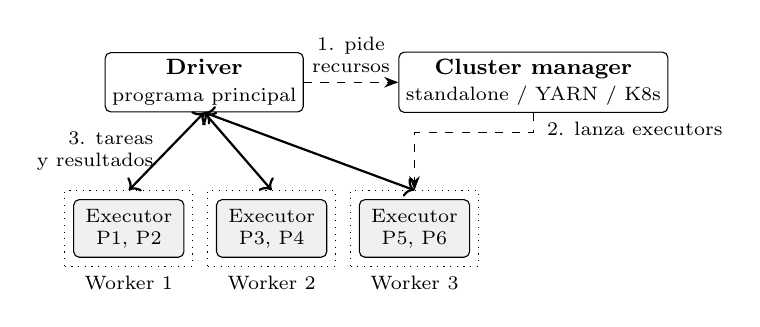
\begin{tikzpicture}[
  font=\footnotesize,
  box/.style={draw, rounded corners=2pt, minimum height=0.7cm, align=center, inner sep=2.5pt},
  exe/.style={draw, rounded corners=2pt, fill=black!6, minimum width=1.4cm, minimum height=0.5cm, align=center, font=\scriptsize},
  arr/.style={-{Stealth[length=1.8mm]}, thick},
  ctl/.style={-{Stealth[length=1.8mm]}, dashed}
]
\node[box, minimum width=2.2cm] (driver) {\textbf{Driver}\\\scriptsize programa principal};
\node[box, minimum width=2.2cm, right=1.2cm of driver] (cm) {\textbf{Cluster manager}\\\scriptsize standalone / YARN / K8s};

\node[exe, below=1.1cm of driver.south west, anchor=north west, xshift=-0.4cm] (e1) {Executor\\P1, P2};
\node[exe, right=0.4cm of e1] (e2) {Executor\\P3, P4};
\node[exe, right=0.4cm of e2] (e3) {Executor\\P5, P6};

\node[draw, dotted, fit=(e1), inner sep=3pt, label={[font=\scriptsize]below:Worker 1}] (w1) {};
\node[draw, dotted, fit=(e2), inner sep=3pt, label={[font=\scriptsize]below:Worker 2}] (w2) {};
\node[draw, dotted, fit=(e3), inner sep=3pt, label={[font=\scriptsize]below:Worker 3}] (w3) {};

\draw[ctl] (driver) -- node[above, font=\scriptsize, align=center] {1. pide\\recursos} (cm);
\draw[ctl] (cm.south) |- ++(0,-0.25) -| (w3.north);
\draw[arr, <->] (driver.south) -- (w2.north);
\draw[arr, <->] (driver.south) -- node[left, font=\scriptsize, align=right, xshift=-1pt] {3. tareas\\y resultados} (w1.north);
\draw[arr, <->] (driver.south) -- (w3.north);
\node[font=\scriptsize, anchor=west] at ($(cm.south)+(0.05,-0.2)$) {2. lanza executors};
\end{tikzpicture}
\caption{Arquitectura de ejecución en Apache Spark. Tras la asignación de recursos por el Cluster Manager, el Driver despacha tareas directamente a los Executors y recolecta resultados.}
\label{fig:arquitectura}
\vspace{-6pt}
\end{figure}

\subsection{Spark MLlib}

MLlib es el componente nativo de Apache Spark destinado al aprendizaje automático escalable~\cite{meng2016mllib}. Provee implementaciones distribuidas de algoritmos de agrupamiento, clasificación, regresión, análisis de componentes principales y recomendación colaborativa. Su ventaja arquitectónica radica en que el mismo código ensayado en un entorno local puede escalarse a miles de núcleos y terabytes de datos sin modificaciones algorítmicas, aprovechando la infraestructura de paralelismo de datos.

\section{Casos de uso y comparación con el modelo relacional}
\label{sec:relacional}

\subsection{Escenarios de aplicación y cargas de trabajo}

Spark está diseñado para cargas analíticas masivas (OLAP, \textit{Online Analytical Processing}) y procesamiento por lotes sobre volúmenes que desbordan un servidor individual. Un escenario representativo es un flujo ETL (\textit{Extract, Transform, Load}) que ingiere terabytes de eventos web o registros transaccionales, aplica desnormalizaciones y agrega métricas para consultas de inteligencia de negocio mediante Spark SQL~\cite{spark-sql}. Otro escenario típico es el entrenamiento distribuido de modelos predictivos y de segmentación con MLlib sobre lagos de datos (\textit{data lakes}). El caso de estudio de K-Means analizado en este trabajo modela la segmentación masiva de usuarios o transacciones a partir de datos consolidados en lagos de datos empresariales.

Por el contrario, Spark no constituye un reemplazo adecuado para motores de bases de datos relacionales en entornos operacionales y transaccionales (OLTP, \textit{Online Transaction Processing}). En escenarios donde se requieren lecturas y modificaciones puntuales de registros individuales con latencias de milisegundos, concurrencia de miles de clientes concurrentes y restricciones estrictas de integridad referencial, los motores relacionales clásicos superan ampliamente a los sistemas distribuidos basados en lotes. Distribuir un conjunto de datos pequeño en un clúster Spark introduce sobrecargas de serialización, red y coordinación que degradan el rendimiento en comparación con una ejecución mono-nodo optimizada.

\subsection{Diferencias y complementariedad arquitectónica}

Spark no es una base de datos: carece de almacenamiento propio dependiente de disco y de mecanismos nativos de transacciones ACID para escrituras atómicas concurrentes a nivel de tupla. Aunque Spark SQL ofrece una sintaxis declarativa idéntica al estándar relacional, las consultas se traducen en planes de transformaciones distribuidas sobre particiones completas de datos~\cite{spark-sql}.

Asimismo, las bases de datos relacionales tradicionales preservan la persistencia e integridad mediante registros de escritura previa (\textit{Write-Ahead Logging}, WAL) y réplicas de almacenamiento~\cite{postgresql-transactions}. Spark, en contraposición, recurre al linaje determinista del DAG para reconstruir particiones perdidas en memoria, delegando la persistencia duradera final al sistema de archivos subyacente (ej. HDFS, Amazon S3).

\begin{table}[t]
\caption{Comparación entre bases de datos relacionales y Apache Spark}
\label{tab:relacional}
\centering
\footnotesize
\begin{tabular}{@{}>{\raggedright\arraybackslash}p{1.7cm}>{\raggedright\arraybackslash}p{2.4cm}>{\raggedright\arraybackslash}p{2.4cm}@{}}
\toprule
\textbf{Dimensión} & \textbf{Base de datos relacional} & \textbf{Apache Spark} \\
\midrule
Propósito central & Transacciones OLTP y consultas operacionales & Procesamiento analítico OLAP y ML distribuido \\
Unidad operativa & Filas, índices B-Tree y tablas relacionales & Particiones distribuidas, RDD y DataFrames \\
Patrón de acceso & Lecturas/escrituras atómicas puntuales indexadas & Escaneo masivo, transformaciones y reducciones \\
Escalabilidad & Vertical predominante (o sharding complejo) & Horizontal elástica sobre clústeres de cómputo \\
Garantías ACID & Integridad referencial y transacciones nativas & Dependientes del sistema de almacenamiento destino \\
Uso de SQL & Consultas sobre esquemas fijos indexados & Optimización de planes masivos con Catalyst \\
\bottomrule
\end{tabular}
\vspace{-5pt}
\end{table}

En la práctica empresarial ambas tecnologías son complementarias: los sistemas relacionales registran el tráfico transaccional continuo y periódicamente vuelcan sus datos a almacenes distribuidos, donde clústeres de Spark ejecutan procesos de agregación, minería y entrenamiento analítico.

\section{K-Means distribuido}
\label{sec:kmeans}

\subsection{Formulación del algoritmo}

Dado un conjunto de $n$ puntos multidimensionales $x_1,\ldots,x_n \in \mathbb{R}^d$ y un número predeterminado $k$ de conglomerados, K-Means busca hallar un conjunto de centroides $\mu_1,\ldots,\mu_k \in \mathbb{R}^d$ que minimice la función de costo de error cuadrático intra-grupo (WSSSE, \textit{Within-Set Sum of Squared Errors}):
\begin{equation}
J = \sum_{i=1}^{n} \min_{j \in \{1,\ldots,k\}} \lVert x_i - \mu_j \rVert^2 .
\label{eq:costo}
\end{equation}

El algoritmo clásico de Lloyd~\cite{lloyd1982,macqueen1967} aproxima numéricamente la solución alternando iterativamente dos fases hasta alcanzar la convergencia:
\begin{enumerate}
\item \textbf{Asignación}: Cada punto $x_i$ se asocia al centroide más próximo según la distancia euclídea:
\begin{equation}
c(i) = \arg\min_{j \in \{1,\ldots,k\}} \lVert x_i - \mu_j \rVert^2 .
\end{equation}
\item \textbf{Actualización}: Se recalculan los $k$ centroides como el baricentro de todos los puntos asignados a cada grupo $j$:
\begin{equation}
\mu_j = \frac{1}{|C_j|} \sum_{i \in C_j} x_i, \quad \text{donde } C_j = \{i : c(i) = j\} .
\end{equation}
\end{enumerate}

Dado que cada iteración reduce monotónicamente o conserva el costo $J$, el algoritmo converge en un número finito de pasos a un mínimo local condicionado por los centroides iniciales.

\subsection{Paralelización mediante estadísticos suficientes}

La fase de asignación exhibe un paralelismo elemental (\textit{embarrassingly parallel}): conociendo los $k$ centroides actuales, cualquier ejecutor puede clasificar sus puntos asignados de manera estrictamente local y sin consultar a otros nodos. En contraste, la fase de actualización requiere consolidar la información global de todas las particiones del clúster.

Transmitir todos los puntos asignados al \textit{driver} anularía las ventajas del procesamiento distribuido. Para evitarlo, cada partición local $p$ calcula para cada grupo $j$ un vector de suma acumulada $S_{p,j} \in \mathbb{R}^d$ y un contador escalar $N_{p,j} \in \mathbb{N}$:
\begin{equation}
S_{p,j} = \sum_{i \in p,\; c(i)=j} x_i, \qquad N_{p,j} = \bigl|\{ i \in p : c(i)=j \}\bigr| .
\end{equation}

El par $(S, N)$ constituye un \textbf{estadístico suficiente}: encapsula toda la información requerida para computar el promedio global exacto. Como la suma vectorial y la suma escalar son operaciones asociativas y conmutativas, pueden reducirse en cualquier orden a lo largo del clúster. Una vez acumuladas las sumas globales, el nuevo centroide se obtiene mediante una única división:
\begin{equation}
\mu_j' = \frac{\sum_p S_{p,j}}{\sum_p N_{p,j}} .
\label{eq:centroide}
\end{equation}

El volumen de datos a transferir por partición se reduce a $k(d+1)$ números en punto flotante, magnitud completamente independiente del número $n$ de registros.

\subsection{El sesgo del promedio de promedios}

Una aproximación errónea recurrente consiste en calcular directamente en cada partición el vector promedio local $\bar{x}_{p,j} = S_{p,j} / N_{p,j}$ y promediar posteriormente dichos vectores en el \textit{driver}. Esta estrategia produce un resultado matemáticamente incorrecto cuando las particiones poseen cardinalidades desiguales en un conglomerado, al ignorar la ponderación $N_{p,j}$. Considérese el caso unidimensional con un punto en $x=10$ en la partición 1 y tres puntos en $x=0$ en la partición 2:
\begin{equation}
\underbrace{\frac{10 + 0}{2} = 5}_{\text{Promedio de promedios (erróneo)}}
\quad\neq\quad
\underbrace{\frac{10 + 0 + 0 + 0}{4} = 2{,}5}_{\text{Promedio real ponderado}} .
\end{equation}

La Tabla~\ref{tab:mensajes} compara tres posibles estrategias de comunicación entre los \textit{executors} y el \textit{driver} durante cada iteración, analizadas para un escenario con $k=3$, $d=2$ y números en punto flotante de 8 bytes (doble precisión).

\begin{table}[t]
\caption{Estrategias de comunicación entre executors y driver}
\label{tab:mensajes}
\centering
\footnotesize
\begin{tabular}{@{}l>{\raggedright\arraybackslash}p{2.3cm}cc@{}}
\toprule
\textbf{Estrategia} & \textbf{Contenido} & \textbf{Volumen} & \textbf{Exacto} \\
\midrule
A (Centralizada) & Puntos completos de partición & $\propto n_p$ (19\,MiB/$10^6$) & Sí \\
B (Promedio local) & Promedio local $\bar{x}_{p,j}$ & 48\,B & No \\
C (Estadístico suf.) & Suma $S_{p,j}$ y conteo $N_{p,j}$ & 72\,B & Sí \\
\bottomrule
\end{tabular}
\vspace{-5pt}
\end{table}

La opción~A es correcta pero traslada todos los registros individuales al \textit{driver}, anulando el beneficio de la computación distribuida y saturando el ancho de banda de red. La opción~B reduce drásticamente el tráfico pero introduce un sesgo matemático inaceptable, ya que no pondera las cardinalidades de cada partición. La opción~C es mínima en volumen de red ($O(kd)$ independiente de $n_p$) y matemáticamente exacta, aplicando el concepto del \textit{combiner} de MapReduce al agrupamiento distribuido.

\subsection{Inicialización e implementación en PySpark MLlib}

Dado que K-Means es sensible a la posición inicial de los centros, Spark implementa el algoritmo \textit{k-means$\|$}~\cite{bahmani2012scalable}, una generalización paralela de \textit{k-means++} que muestrea múltiples centroides candidatos simultáneamente en $O(\log n)$ pasadas sobre el clúster. Los parámetros centrales del estimador \texttt{pyspark.ml.clustering.KMeans} son la cantidad de grupos \texttt{k}, la tolerancia de convergencia \texttt{tol}, el límite de iteraciones \texttt{maxIter} y la semilla aleatoria \texttt{seed}~\cite{spark-mllib}. El Listado~\ref{lst:pyspark} exhibe un flujo de entrenamiento básico.

\begin{lstlisting}[language=Python, caption={K-Means con PySpark y MLlib}, label={lst:pyspark}]
from pyspark.ml.clustering import KMeans
from pyspark.ml.feature import VectorAssembler
df = spark.read.csv("clientes.csv", header=True, inferSchema=True)
vec = VectorAssembler(inputCols=["x", "y"], outputCol="features")
datos = vec.transform(df).cache()
modelo = KMeans(k=3, maxIter=12, seed=1).fit(datos)
print(modelo.clusterCenters())
print(modelo.summary.trainingCost)  # WSSSE
\end{lstlisting}

La invocación a \texttt{cache()} resulta determinante: asegura que las transformaciones se computen una sola vez y residan en la RAM de los ejecutores, acelerando drásticamente las iteraciones sucesivas.

\section{Tolerancia a fallos y rendimiento}
\label{sec:fallos}

\subsection{Recuperación por linaje}

En clústeres a gran escala compuestos por decenas o cientos de nodos, las fallas transitorias o definitivas de hardware son eventos esperados. Hadoop mitiga este fenómeno replicando bloques de datos tres veces en disco local~\cite{shvachko2010hdfs}. Spark, en contrapartida, evita la costosa replicación en memoria de estructuras intermedias apoyándose en el linaje del RDD~\cite{zaharia2012rdd}. Cada RDD mantiene información de solo lectura sobre sus transformaciones ascendentes. Si un nodo ejecutor cae durante la iteración 10 de K-Means, el \textit{driver} detecta la pérdida de la tarea y la reasigna a otro ejecutor disponible, quien reconstruye exclusivamente la partición afectada releyendo su porción de la fuente base persistente.

\subsection{Tareas rezagadas y ejecución especulativa}

La velocidad de una etapa paralela está gobernada por su tarea más lenta (\textit{straggler}). Los rezagados surgen por degradación de discos locales, contención de red o competencia de hilos. Dean y Ghemawat propusieron neutralizar este cuello de botella despachando tareas duplicadas de respaldo (\textit{backup tasks})~\cite{dean2004mapreduce}. Spark implementa esta estrategia mediante el parámetro \texttt{spark.speculation}. Cuando se habilita, el sistema monitorea la duración de las tareas y relanza una copia especulativa en otro nodo si una tarea en ejecución supera un múltiplo configurado (\texttt{spark.speculation.multiplier}) de la mediana de su etapa, adoptando los resultados de la primera instancia que finalice con éxito~\cite{spark-config}.

\subsection{Comparación analítica entre Spark y Hadoop}

Sea $r$ el costo temporal de leer una partición desde disco, $c$ el tiempo de cálculo local por iteración y $w$ el tiempo de volcar resultados intermedios a almacenamiento persistente. Para un algoritmo que requiere $m$ iteraciones sucesivas, el costo acumulado de Hadoop MapReduce se modela como:
\begin{equation}
T_{\text{Hadoop}} \approx m\,(r + c + w),
\end{equation}
mientras que Spark, preservando los datos en memoria tras la primera lectura, requiere:
\begin{equation}
T_{\text{Spark}} \approx r + m\,c .
\end{equation}

En aplicaciones iterativas donde la I/O domina sobre el cómputo ($r + w \gg c$), la aceleración teórica crece casi proporcionalmente a $m$. Investigaciones empíricas reportan reducciones de tiempo de hasta un orden de magnitud a favor de Spark en algoritmos de aprendizaje automático~\cite{zaharia2012rdd}. La Tabla~\ref{tab:comparacion} sintetiza las diferencias paradigmáticas.

\begin{table}[t]
\caption{Comparación entre Hadoop MapReduce y Apache Spark}
\label{tab:comparacion}
\centering
\footnotesize
\begin{tabular}{@{}>{\raggedright\arraybackslash}p{1.8cm}>{\raggedright\arraybackslash}p{2.5cm}>{\raggedright\arraybackslash}p{2.5cm}@{}}
\toprule
\textbf{Característica} & \textbf{Hadoop MapReduce} & \textbf{Apache Spark} \\
\midrule
Datos entre pasos & Disco distribuido (HDFS) & Memoria RAM (\texttt{cache}) \\
Modelo de cómputo & Map y Reduce acoplados & Grafo acíclico (DAG) flexible \\
Tolerancia a fallos & Replicación física de bloques & Linaje determinista y recálculo \\
Soporte iterativo & Un trabajo aislado por paso & Un único contexto de ejecución \\
APIs soportadas & Java & Python, Scala, SQL, R, Java \\
\bottomrule
\end{tabular}
\vspace{-5pt}
\end{table}

\section{Machine Learning a escala: Arquitectura, Pipelines y Optimización}
\label{sec:mllib-avanzado}

La paralelización básica descrita en la Sección~\ref{sec:kmeans} asume una comunicación plana hacia el maestro. Sin embargo, en despliegues con petabytes de datos y miles de particiones, la arquitectura debe resolver problemas de saturación de red, orquestación de características, optimización de hardware y asimetría de particiones.

\subsection{Comunicación distribuida y agregación en árbol}

Cuando un clúster opera con miles de particiones $P$, enviar los vectores de estadísticos $(S_{p,j}, N_{p,j})$ directamente al \textit{driver} origina un cuello de botella $O(P)$ de conexiones y tráfico de red entrante sobre un único puerto, desencadenando agotamiento de memoria (\textit{Out Of Memory}, OOM) y serialización forzada de las adiciones.

Para resolver esta vulnerabilidad, Spark MLlib implementa la \textbf{agregación jerárquica en árbol} (\texttt{treeAggregate} y \texttt{treeReduce})~\cite{meng2016mllib}. En lugar de transferir todos los mensajes a un punto central, la reducción se estructura en niveles sucesivos con una profundidad configurable $h \ge 2$ (\texttt{depth}), como se ilustra en la Fig.~\ref{fig:tree-aggregate}.

\begin{figure}[t]
\centering
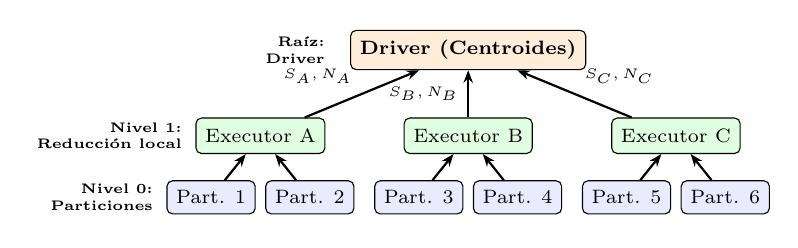
\begin{tikzpicture}[
  font=\scriptsize,
  part/.style={draw, rounded corners=2pt, fill=blue!8, minimum width=0.95cm, minimum height=0.42cm, align=center},
  inter/.style={draw, rounded corners=2pt, fill=green!12, minimum width=1.3cm, minimum height=0.45cm, align=center},
  root/.style={draw, rounded corners=2pt, fill=orange!15, minimum width=2.0cm, minimum height=0.5cm, align=center, font=\scriptsize\bfseries},
  arr/.style={-{Stealth[length=1.6mm]}, thick}
]
% Nivel 0: Particiones
\node[part] (p1) {Part. 1};
\node[part, right=0.12cm of p1] (p2) {Part. 2};
\node[part, right=0.25cm of p2] (p3) {Part. 3};
\node[part, right=0.12cm of p3] (p4) {Part. 4};
\node[part, right=0.25cm of p4] (p5) {Part. 5};
\node[part, right=0.12cm of p5] (p6) {Part. 6};

% Nivel 1: Agregadores intermedios
\node[inter, above=0.55cm of $(p1)!0.5!(p2)$] (i1) {Executor A};
\node[inter, above=0.55cm of $(p3)!0.5!(p4)$] (i2) {Executor B};
\node[inter, above=0.55cm of $(p5)!0.5!(p6)$] (i3) {Executor C};

% Nivel 2: Driver
\node[root, above=0.6cm of i2] (drv) {Driver (Centroides)};

% Flechas nivel 0 -> 1
\draw[arr] (p1) -- (i1);
\draw[arr] (p2) -- (i1);
\draw[arr] (p3) -- (i2);
\draw[arr] (p4) -- (i2);
\draw[arr] (p5) -- (i3);
\draw[arr] (p6) -- (i3);

% Flechas nivel 1 -> 2
\draw[arr] (i1) -- node[above left, font=\tiny] {$S_A, N_A$} (drv);
\draw[arr] (i2) -- node[left, font=\tiny] {$S_B, N_B$} (drv);
\draw[arr] (i3) -- node[above right, font=\tiny] {$S_C, N_C$} (drv);

% Etiquetas de nivel
\node[left=0.05cm of p1, font=\tiny\bfseries, align=right] {Nivel 0:\\Particiones};
\node[left=0.05cm of i1, font=\tiny\bfseries, align=right] {Nivel 1:\\Reducción local};
\node[left=0.2cm of drv, font=\tiny\bfseries, align=right] {Raíz:\\Driver};
\end{tikzpicture}
\caption{Agregación jerárquica con \texttt{treeAggregate} en Spark MLlib. Los ejecutores intermedios combinan estadísticos suficientes en paralelo antes de transmitirlos al nodo maestro, evitando saturar la interfaz de red del \textit{driver}.}
\label{fig:tree-aggregate}
\vspace{-6pt}
\end{figure}

En el nivel 0, cada ejecutor consolida las estadísticas de sus particiones locales. En los niveles intermedios, un grupo de ejecutores actúa como agregador de un factor de ramificación $b = \lceil P^{1/h} \rceil$ de particiones hijas. Este esquema garantiza que:
\begin{itemize}
\item La cantidad de mensajes que ingresan al \textit{driver} disminuye desde $O(P)$ hasta $O(P^{1/h})$.
\item El cómputo aritmético de suma vectorial se ejecuta en paralelo entre múltiples núcleos distribuidos.
\item La latencia total de agregación escala de manera logarítmica respecto al volumen de particiones.
\end{itemize}

\subsection{Canalizaciones de Machine Learning (ML Pipelines)}

En la práctica industrial de macrodatos, la fase de ajuste del modelo suele representar menos del 20\,\% del cómputo; el preprocesamiento, escalamiento, imputación y codificación de atributos acaparan el resto de la carga. La API basada en DataFrames (\texttt{pyspark.ml}) estandariza estos flujos de trabajo mediante tres abstracciones fundamentales:

\begin{itemize}
\item \textbf{Transformer}: Algoritmo que recibe un DataFrame y produce un nuevo DataFrame derivado (añadiendo columnas de características, vectores densos o predicciones). Operan aplicando transformaciones fila por fila con dependencias estrechas, procesándose en paralelo local sin originar transferencias por \textit{shuffle}.
\item \textbf{Estimator}: Algoritmo parametrizado que implementa el método \texttt{fit()} sobre un DataFrame para aprender patrones de los datos, produciendo como resultado un \textit{Transformer} entrenado.
\item \textbf{Pipeline}: Grafo lineal ordenado que encadena múltiples transformadores y estimadores. Garantiza la consistencia del flujo, erradica la fuga de datos (\textit{data leakage}) entre conjuntos de entrenamiento y evaluación y facilita la exportación atómica del modelo a producción.
\end{itemize}

El Listado~\ref{lst:pipeline} muestra una canalización distribuida completa que realiza ensamblado vectorial, escalamiento y entrenamiento de K-Means, junto con su posterior evaluación de calidad mediante el coeficiente Silhouette.

\begin{lstlisting}[language=Python, caption={Canalización completa de Machine Learning con PySpark}, label={lst:pipeline}]
from pyspark.ml import Pipeline
from pyspark.ml.feature import VectorAssembler, StandardScaler
from pyspark.ml.clustering import KMeans
from pyspark.ml.evaluation import ClusteringEvaluator

# Ingestion columnar Parquet y preparacion distribuida
df = spark.read.parquet("hdfs:///datos/clientes.parquet")
vec = VectorAssembler(inputCols=["ingreso", "antiguedad", "gastos"], outputCol="vec")
std = StandardScaler(inputCol="vec", outputCol="features", withMean=True, withStd=True)

# Definicion y ajuste del Pipeline con estimador KMeans
kmeans = KMeans(k=4, initMode="k-means||", maxIter=25, seed=42)
pipeline = Pipeline(stages=[vec, std, kmeans])
modelo = pipeline.fit(df)

# Evaluacion distribuida con metrica Silhouette
pred = modelo.transform(df)
score = ClusteringEvaluator(metricName="silhouette").evaluate(pred)
print(f"Silhouette = {score:.4f}")
\end{lstlisting}

\subsection{El motor de optimización: Catalyst y Project Tungsten}

El elevado rendimiento de Spark sobre grandes volúmenes de datos descansa sobre dos componentes internos de su motor relacional y analítico~\cite{armbrust2015sparksql}:

\textbf{Catalyst Optimizer}: Motor de optimización extensible que aplica álgebra relacional sobre árboles sintácticos de operaciones en cuatro etapas consecutivas:
\begin{enumerate}
\item \textit{Análisis}: Resuelve identificadores de columnas, tipos y esquemas contra el catálogo.
\item \textit{Optimización lógica}: Aplica reglas canónicas deterministas, destacando el empuje de predicados (\textit{predicate pushdown}) que filtra registros directamente en el formato de almacenamiento (ej. omitiendo bloques en archivos Parquet sin cargarlos a memoria) y la poda de proyecciones (\textit{column pruning}) para ignorar columnas redundantes.
\item \textit{Optimización física}: Evalúa planes de ejecución mediante modelos de costo (CBO), seleccionando automáticamente estrategias eficientes como transformar uniones costosas en \textit{Broadcast Hash Joins} cuando una tabla es pequeña, eliminando la etapa de \textit{shuffle}.
\item \textit{Generación de código}: Traduce partes del plan optimizado a \textit{bytecode} nativo de Java para su ejecución inmediata.
\end{enumerate}

\textbf{Project Tungsten}: Rediseño de bajo nivel enfocado en optimizar el cómputo a nivel de CPU y memoria física, eliminando la sobrecarga intrínseca de la máquina virtual Java (JVM):
\begin{itemize}
\item \textit{Memoria Off-Heap y formato binario}: Spark gestiona memoria en formato compacto (\texttt{UnsafeRow}), eliminando encabezados de objetos Java (16--24 bytes por tupla) y pausas de recolección de basura (\textit{GC pauses}).
\item \textit{Whole-Stage Code Generation}: Sintetiza en tiempo de ejecución bucles cerrados en Java plano que compilan cadenas completas de operadores, manteniendo datos en los registros y cachés L1/L2/L3 del procesador.
\end{itemize}

\subsection{Desafíos operativos: Sesgo de datos y gestión de Shuffle}

En entornos productivos, el rendimiento del clúster puede degradarse drásticamente si no se gestionan adecuadamente los cuellos de botella de particionamiento~\cite{spark-tuning}:

\textbf{Sesgo de datos (\textit{Data Skew})}: Se manifiesta cuando una distribución no uniforme en las claves de particionamiento concentra una proporción masiva de registros en un único nodo. El ejecutor afectado se convierte en un cuello de botella que retarda la culminación de toda la etapa paralela. Para contrarrestarlo se aplican dos técnicas:
\begin{enumerate}
\item \textit{Salting}: Adición de un prefijo o sufijo aleatorio uniforme $s \in [0, S-1]$ a las claves problemáticas, permitiendo repartir los registros en $S$ subparticiones durante la primera agregación y unificar los resultados mediante una reducción posterior.
\item \textit{Adaptive Query Execution (AQE)}: Característica introducida en versiones recientes que analiza estadísticas en tiempo de ejecución al concluir cada etapa de \textit{shuffle}, subdividiendo automáticamente particiones anómalas sin requerir reescritura manual del código.
\end{enumerate}

\textbf{Desbordamiento a disco (\textit{Shuffle Spill})}: Durante las etapas de \textit{shuffle}, los ejecutores ordenan y reagrupan grandes volúmenes de datos. Si la memoria asignada a la ejecución (\texttt{spark.memory.fraction}) es desbordada, Spark escribe temporalmente los fragmentos excedentes a disco local sin compresión (\textit{spill to disk}), penalizando la velocidad entre un factor de 10x y 50x. Se previene calibrando el número de particiones (\texttt{spark.sql.shuffle.partitions}, buscando bloques de 100 a 200~MiB) y configurando el serializador binario Kryo (\texttt{KryoSerializer}) en sustitución de la serialización nativa de Java.

\section{Conclusiones}
\label{sec:conclusiones}

El procesamiento distribuido sobre macrodatos constituye una necesidad técnica cuando el volumen, la velocidad y la dimensionalidad de la información desbordan la capacidad de un servidor individual. Apache Spark superó las limitaciones de I/O en disco del modelo MapReduce al introducir colecciones inmutables en memoria con tolerancia a fallos basada en linaje determinista, posibilitando la ejecución eficiente de algoritmos iterativos.

El estudio formal de K-Means demostró que el escalamiento horizontal efectivo depende de una formulación algorítmica adecuada: el uso de estadísticos suficientes reduce la transmisión de red a una magnitud independiente del número de instancias, mientras que la agregación jerárquica en árbol (\texttt{treeAggregate}) previene la saturación del nodo maestro al distribuir el cómputo de consolidación.

Asimismo, se evidenció que los sistemas de gestión de bases de datos relacionales y los motores distribuidos como Spark cumplen roles complementarios. Mientras que los primeros ofrecen garantías transaccionales ACID y latencias de milisegundos en operaciones de negocio operacionales (OLTP), Spark provee la infraestructura analítica masiva y elástica (OLAP) requerida para la ingeniería de datos y el entrenamiento de modelos de aprendizaje automático a gran escala.

Finalmente, la consecución de una alta eficiencia en producción exige optimizaciones a nivel de motor de ejecución y control de infraestructura. Los avances provistos por el optimizador Catalyst y Project Tungsten permiten aprovechar al máximo las capacidades físicas del hardware moderno; sin embargo, el diseño adecuado de esquemas de particionamiento, la mitigación del sesgo de datos (\textit{data skew}) y el control del desbordamiento en el \textit{shuffle} siguen siendo responsabilidades cardinales de la ingeniería de datos para garantizar la escalabilidad lineal en el procesamiento masivo.

\begin{thebibliography}{99}
\setlength{\itemsep}{0pt}
\setlength{\parskip}{0pt}

\bibitem{dean2004mapreduce}
J.~Dean and S.~Ghemawat, ``MapReduce: Simplified data processing on large clusters,'' in \textit{Proc. 6th USENIX Symp. Operating Systems Design and Implementation (OSDI)}, San Francisco, CA, USA, 2004, pp.~137--150.

\bibitem{shvachko2010hdfs}
K.~Shvachko, H.~Kuang, S.~Radia, and R.~Chansler, ``The Hadoop distributed file system,'' in \textit{Proc. IEEE 26th Symp. Mass Storage Systems and Technologies (MSST)}, 2010, pp.~1--10.

\bibitem{zaharia2010spark}
M.~Zaharia, M.~Chowdhury, M.~J. Franklin, S.~Shenker, and I.~Stoica, ``Spark: Cluster computing with working sets,'' in \textit{Proc. 2nd USENIX Workshop Hot Topics in Cloud Computing (HotCloud)}, 2010.

\bibitem{zaharia2012rdd}
M.~Zaharia \textit{et al.}, ``Resilient distributed datasets: A fault-tolerant abstraction for in-memory cluster computing,'' in \textit{Proc. 9th USENIX Symp. Networked Systems Design and Implementation (NSDI)}, San Jose, CA, USA, 2012, pp.~15--28.

\bibitem{zaharia2016unified}
M.~Zaharia \textit{et al.}, ``Apache Spark: A unified engine for big data processing,'' \textit{Commun. ACM}, vol.~59, no.~11, pp.~56--65, 2016.

\bibitem{meng2016mllib}
X.~Meng \textit{et al.}, ``MLlib: Machine learning in Apache Spark,'' \textit{J. Mach. Learn. Res.}, vol.~17, no.~34, pp.~1--7, 2016.

\bibitem{vavilapalli2013yarn}
V.~K. Vavilapalli \textit{et al.}, ``Apache Hadoop YARN: Yet another resource negotiator,'' in \textit{Proc. 4th ACM Symp. Cloud Computing (SoCC)}, 2013, pp.~5:1--5:16.

\bibitem{lloyd1982}
S.~Lloyd, ``Least squares quantization in PCM,'' \textit{IEEE Trans. Inf. Theory}, vol.~28, no.~2, pp.~129--137, 1982.

\bibitem{macqueen1967}
J.~MacQueen, ``Some methods for classification and analysis of multivariate observations,'' in \textit{Proc. 5th Berkeley Symp. Mathematical Statistics and Probability}, vol.~1, 1967, pp.~281--297.

\bibitem{bahmani2012scalable}
B.~Bahmani, B.~Moseley, A.~Vattani, R.~Kumar, and S.~Vassilvitskii, ``Scalable k-means++,'' \textit{Proc. VLDB Endowment}, vol.~5, no.~7, pp.~622--633, 2012.

\bibitem{armbrust2015sparksql}
M.~Armbrust \textit{et al.}, ``Spark SQL: Relational data processing in Spark,'' in \textit{Proc. 2015 ACM SIGMOD Int. Conf. Management of Data}, Melbourne, Australia, 2015, pp.~1383--1394.

\bibitem{spark-cluster}
The Apache Software Foundation, ``Cluster mode overview,'' \textit{Apache Spark Documentation}. [Online]. Available: \url{https://spark.apache.org/docs/latest/cluster-overview.html} (accedido: nov. 2026).

\bibitem{spark-mllib}
The Apache Software Foundation, ``Clustering --- K-means,'' \textit{Apache Spark MLlib Guide}. [Online]. Available: \url{https://spark.apache.org/docs/latest/ml-clustering.html} (accedido: nov. 2026).

\bibitem{spark-sql}
The Apache Software Foundation, ``Spark SQL, DataFrames and Datasets Guide,'' \textit{Apache Spark Documentation}. [Online]. Available: \url{https://spark.apache.org/docs/latest/sql-programming-guide.html} (accedido: nov. 2026).

\bibitem{spark-config}
The Apache Software Foundation, ``Spark configuration,'' \textit{Apache Spark Documentation}. [Online]. Available: \url{https://spark.apache.org/docs/latest/configuration.html} (accedido: nov. 2026).

\bibitem{spark-tuning}
The Apache Software Foundation, ``Tuning Spark,'' \textit{Apache Spark Documentation}. [Online]. Available: \url{https://spark.apache.org/docs/latest/tuning.html} (accedido: nov. 2026).

\bibitem{postgresql-transactions}
The PostgreSQL Global Development Group, ``Transactions,'' \textit{PostgreSQL Documentation}. [Online]. Available: \url{https://www.postgresql.org/docs/current/tutorial-transactions.html} (accedido: nov. 2026).

\end{thebibliography}

\end{document}
